\documentclass[10pt,a4paper]{jarticle} %参考文献改ページ防ぐためにjarticleにしてるよ
\usepackage[top=20truemm,bottom=20truemm,left=20truemm,right=20truemm]{geometry}
\usepackage[dvipdfmx]{graphicx}
\usepackage{here}
\usepackage{amsmath}
\usepackage{url}
\usepackage{cases}
\usepackage{braket}
\usepackage{caption} %図表キャプションまわり
\captionsetup[figure]{format=plain, labelformat=simple, labelsep=space, font=footnotesize}
\captionsetup[table]{format=plain, labelformat=simple, labelsep=space, font=small}
%\renewcommand{\bibname}{} %jreportではデフォルトで関連図書とかになる

\begin{document}
\begin{center}
\bf{\LARGE 熱電変換材料と性能指数$Z$}
\end{center}
\begin{flushright}
N. H. Shimada
\end{flushright}

頑張って図書いたので公開します。熱電変換材料の性能指数Zの表式を導出する。性能指数は、「流れる電気エネルギー/流れる熱エネルギー」によって評価される無次元量である。
\begin{figure}[ht]
\centering  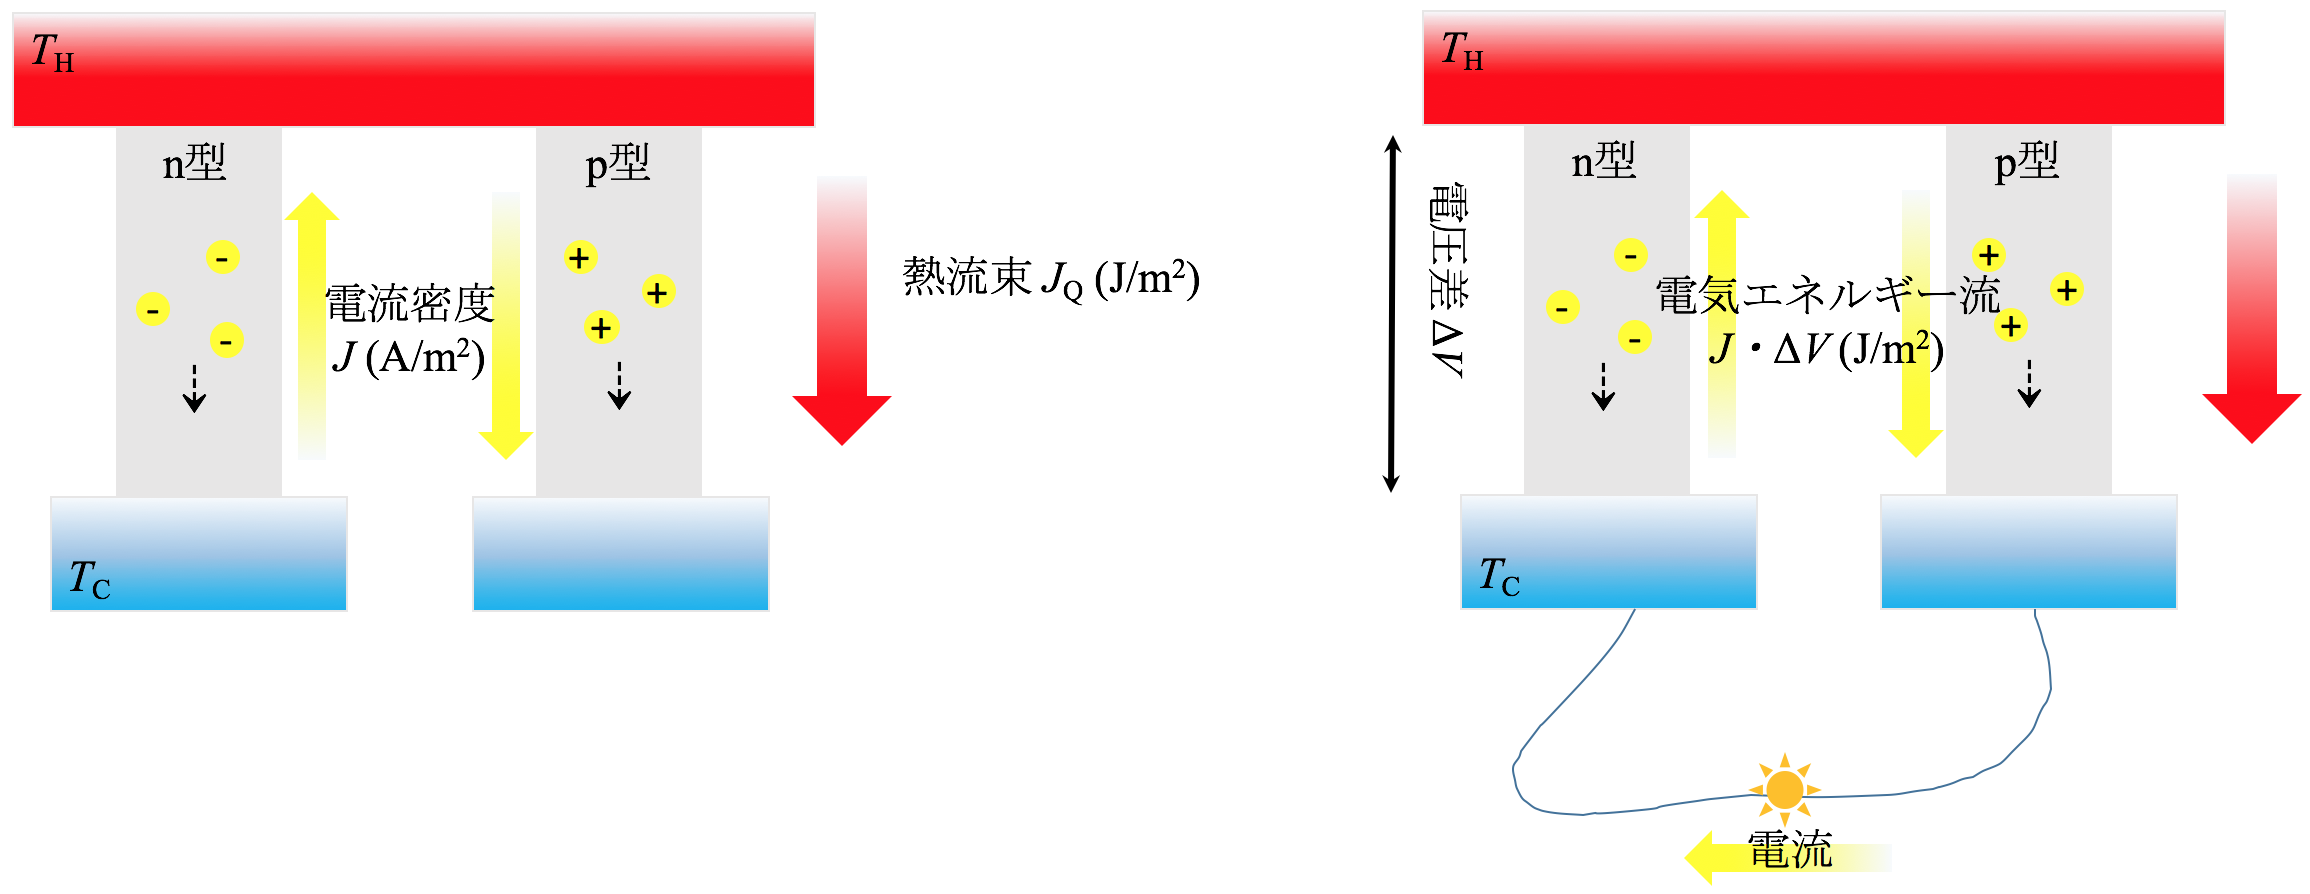
\includegraphics[width=15cm]{trans_all.png} 
\caption{熱電変換材料の模式図。(左図)高温側と低温側をn型p型半導体で接続すると図のようにキャリア流と熱流が発生する。(右図)低温側の2つの素子を電気回路で繋ぐことで、電流を取り出すことが出来る。}
\label{Si_lod}
\end{figure}\\
図のように、高温側($T_H$)と低温側($T_C \equiv T_H - \Delta T$)がn型とp型2つの半導体によって接続されているような熱電変換材料を考える。この時、高温側から低温側へは熱勾配に基づいて熱流$J_Q$(J/$\mathrm{m}^2$)が発生する(Fourier則)。熱伝導率$\kappa$で一定値とすると、次のような関係式が成立する。
\begin{equation}
| J_Q |= \kappa \Delta T
\label{eq:j_q} \end{equation}
熱と同様に、2つの半導体中のキャリアはそれぞれ高温側から低温側へと流れる。この時両端に生じる電圧差$\Delta V $は、ゼーベック係数を$S$(一定値)として、次のように表せる。
\begin{equation}
\Delta V = S \Delta T
\end{equation}
この電圧に応じて流れる電流密度$J(\mathrm{A/m^2})$は、電気伝導度$\sigma$とすると、
\begin{equation}
J = \sigma \Delta V
\end{equation}
であり、電流により運ばれる電気的エネルギー$J \cdot \Delta V (\mathrm{J/m^2})$は、
\begin{eqnarray}
J \cdot \Delta V &=& \sigma (\Delta V)^2 \\
&=& \sigma S^2 (\Delta T)^2
\label{eq:jdelV} \end{eqnarray}
式(\ref{eq:j_q})と式(\ref{eq:jdelV})より、熱電変換材料の変換指数$Z \Delta T$ (電気エネルギー/熱エネルギー)は、
\begin{eqnarray}
Z\Delta T &=& \frac{J \cdot \Delta V}{| J_Q |}\\
&=& \frac{\sigma S^2 (\Delta T)^2}{\kappa \Delta T} \\
&=& \frac{\sigma S^2 \Delta T}{\kappa}
\end{eqnarray}
よって、
\begin{eqnarray}
Z = \frac{\sigma S^2}{\kappa}
\end{eqnarray}


\end{document}